\subsection{Probabilistic modelling} \label{section:probabilistic_modelling}

A scientific model is a simple theoretical representation of a complex natural phenomenon to allow the systematic study of its behaviour. The general idea is that if a model is able to explain some observations, it might be capturing its true underlying laws and can therefore be used to make future predictions.
In particular, statistical models are a powerful abstraction of nature. They consist of a set of observed variables and a set of (hidden) parameters. The procedure of fitting the parameters using a set of observations is called inference or learning.

One of the major challenges of inference when dealing with real data sets is the distinction between signal and noise. An ideal model should learn only the information relevant to gain explanatory power while disregarding the noise. However, this is a non-trivial task in most practical situations. Very complex models will tend to overfit the training data, capturing large amounts of noise and consequently leading to a bad generalisation performance to independent data sets. On the other hand, simplistic models will fit the data poorly, leading to poor explanatory power.

The ideas above can be formalised using the framework of probability and statistics.

\subsection{Maximum likelihood inference} \label{section:maximum_likelihood}

A common approach is to define a statistical model of the data $\bfY$ with a set of parameters $\btheta$ that define a probability distribution $p(\bfY|\btheta)$, called the likelihood function. A simple approach to fit a model is to estimate the parameters $\hat{\btheta}$ that maximise the likelihood:
\[
	\hat{\btheta} = \argmax_{\btheta} p(\bfY|\btheta)
\]
This process is called maximum likelihood learning \cite{Stigler2008,Bishop2006,Murphy}. However, in this setting there is no penalisation for model complexity, making maximum likelihood solutions can overfit when the data is relatively sparse. Generalisations that account for model complexity have been proposed that include regularising terms that shrink parameters to small values. However, these are often particular cases of the more general framework of Bayesian statistics \cite{Hastie,Bishop2006,Murphy}.

\subsection{Bayesian inference}  \label{section:bayesian_inference}
In the Bayesian framework, the parameters themselves are treated as random unobserved variables and we aim to obtain probability distributions for $\btheta$, rather than a single point estimate. To do so, prior beliefs are introduced into the model by specifying a prior probability distribution $p(\btheta)$. Then, using Bayes' theorem \cite{Bayes1763}, the prior hypothesis is updated based on the observed data $\bfY$ by means of the likelihood $p(\bfY|\btheta)$ function, which yields a posterior distribution over the parameters:
\[
	p(\btheta|\bfY) = \frac{p(\bfY|\btheta) p(\btheta)}{p(\bfY)}
\]
where $p(\bfY)$ is a constant term called the marginal likelihood, or model evidence \cite{Bishop2006,Murphy}.\\
The choice of the prior distribution is a key part of Bayesian inference and captures beliefs about the distribution of a variable before the data is taken into account. With asymptotically large sample sizes, the choice of prior has negligible effects on the posterior estimates, but it becomes critical with sparse data \cite{Bishop2006,Murphy,Gelman2013}.

There are two common considerations when defining the prior distributions. The first relates to the incorporation of subjective information, or predefined assumptions, into the model. For example, one could adapt the prior distribution to match the results from previous experiments (i.e. an informative prior). Alternatively, if no information is available one could set set uninformative priors by following maximum entropy principles \cite{Jaynes1968}.

The second strategy is based on convenient mathematical properties to make inference tractable. If the likelihood and the prior distributions do not belong to the same family of probability distributions (they are not conjugate) then inference becomes more problematic \cite{Raiffa1961,Bishop2006,Murphy,Gelman2013}. The existence of conjugate priors is one of the major reasons that justify the widespread use of exponential family distributions in Bayesian models \cite{Gelman2013}.

Again, the essential point of Bayesian inference is that an entire posterior probability distribution is obtained for each unobserved variable. This has the clear advantage of naturally handling uncertainity in the estimation of parameters. For instance, when making predictions, a fully Bayesian approach attempts to integrate over all possible values of all unobserved varaibles, effectively propagating uncertainity across multiple layers of the model. Nevertheless, this calculation is sometimes intractable and one has to resort to point estimates \cite{Bishop2006,Murphy,Gelman2013}. The simplest approximation to the posterior distribution is to use its mode, which leads to the maximum a posteriori (MAP) estimate:
\[
	\hat{\btheta} = \argmax_{\btheta} p(\btheta) p(\bfY|\btheta) 
\]
This is similar to the maximum likelihood objective function, but with the addition of a term $p(\btheta)$. When the prior distribution is well chosen, this term penalises for model complexity. Therefore, in contrast to standard (non-penalised) maximum likelihood inference, Bayesian approaches naturally handle the problem of model complexity and overfitting \cite{Bishop2006,Murphy,Gelman2013}. At the limit of infinite observations, the influence of the prior to the posterior is negligible and the MAP estimate converges towards the Maximum likelihood estimate, hence providing a rational link between the two inference frameworks.

\subsubsection{Deterministic approaches for Bayesian inference} \label{section:deterministic_bayesian_inference}
The central task in Bayesian inference is the direct evaluation of the posterior distributions and/or the computation of expectations with respect to the posterior distributions. In sufficiently complex models, closed-form solutions are not available and one has to resort to approximation schemes, which broadly fall into two classes: stochastic or deterministic \cite{Gelman2013,Blei2016}. 

Stochastic approaches hinge on the generation of samples from the posterior distribution via a Markov Chain Monte Carlo (MCMC) framework. Such techniques have the appealing property of generating exact results at the asymptotic limit of infinite computational resources. However, in practice, sampling approaches are computationally demanding and suffer from limited scalability to large data sets \cite{Blei2016}. \\
In contrast, deterministic approaches are based on analytical approximations to the posterior distribution, which often lead to biased results. Yet, given the appropriate settings, these approaches are potentially much faster and scalable to large applications \cite{Bishop2006,Murphy,Blei2016}.

% \paragraph{Laplace approximation}% \label{section:laplace_approximation}
% The Laplace approximation is probably the simplest of the deterministic tecniques, where the aim is to construct a Gaussian approximation around the mode of the true posterior distribution using a second-order Taylor expansion \cite{Bishop2006,Murphy}.\\
% Suppose $\bfX$ contains all unobserved variables. The true posterior distribution can be written as:
% \[
% p(\bfX) = \frac{f(\bfX)}{Z}
% \]
% where $f(\bfX)$ is a function that depends on the unobserved variables and $Z$ is an unknown normalisation constant to ensure that $\int p(\bfX) d\bfX = 1$.

% The second-order Taylor expansion of $\log f(\bfX)$ centered around its (known) mode $\hat{\bfX}$ is: 
% \[
% 	\log f(\bfX) \approx \log f(\hat{\bfX}) - \frac{1}{2} (\bfX-\hat{\bfX})^T \bfA (\bfX-\hat{\bfX})
% \]
% where $\bfA = \nabla^2 \log f(\hat{\bfX})$ is the Hessian matrix of $\log f(\bfX)$ evaluated at $\hat{\bfX}$.\\
% Notice three things. First, the first-order term of the Taylor expansion is zero because $\hat{\bfX}$ is a stationary point. Second, the $\log$ function is monotonically increasing and therefore a maximum of $\log f(\bfX)$ is also a maximum of $f(\bfX)$. Third, the mode of the posterior $p(\bfX)$ must be known, which requires the use of (complex) optimisation algorithms.\\
% Taking the exponential in both sides:
% \[
% 	f(\bfX) \approx f(\hat{\bfX}) \exp\{ -\frac{1}{2} (\bfX-\hat{\bfX})^T \bfA (\bfX-\hat{\bfX}) \}
% \]
% which leads to the following multivariate Gaussian distribution approximation $q(\bfX) = \Ndist{\bfX}{\hat{\bfX},\bfA}$:
% \[
% 	q(\bfX) = \frac{\mid A \mid^{1/2}}{(2\pi^{d/2})} \exp\{ -\frac{1}{2} (\bfX-\hat{\bfX})^T \bfA (\bfX-\hat{\bfX}) \}
% \]
% where $d$ is the number of unobserved variables. \\
% Despite its simplicity, the Laplace approximation is a useful strategy that has been successfully applied in practice. Nonetheless, this approximation has notable caveats: first, is limited by its own local definition, ignoring all the density beyond the mode of the posterior. Second, it does not apply to discrete variables. Third, the inversion of the Hessian is very expensive in high-dimensional settings.
% 	% More sophisticated generalisations of the Laplace approximation have also been proposed \cite{Rue2009}
% 	% To-do: check where does the inverse appear

\subsection{Variational inference}  \label{section:variational_inference}

Variational inference is a deterministic family of methods that have been receiving widespread attention due to a positive balance between accuracy, speed, and ease of use \cite{Blei2016, Zhang2017}. The core framework is derived below.

In variational inference the true (but intractable) posterior distribution $p(\bfX|\bfY)$ is approximated by a simpler (variational) distribution $q(\bfX|\bTheta)$ where $\bTheta$ are the corresponding parameters. The parameters, which we will omit from the notation, need to be tuned to obtain the closest approximation to the true posterior.\\
The distance between the true distribution and the variational distribution is calculated using the KL divergence:
\[
\KL(q(\bfX)||p(\bfX|\bfY)) = - \int q(\bfX) \log \frac{p(\bfX|\bfY)}{q(\bfX)}
\]
Note that the KL divergence is not a proper distance metric, as it is not symmetric. In fact, using the reverse KL divergence $\KL(q(\bfX)||p(\bfY|\bfX))$ defines a different inference framework called expectation propagation \cite{Minka2001}.

If we allow any possible choice of $q(\bfX)$, then the minimum of this function occurs when $q(\bfX)$ equals the true posterior distribution $p(\bfX|\bfY)$. Nevertheless, since the true posterior is intractable to compute, this does not lead to any simplification of the problem. Instead, it is necessary to consider a restricted family of distributions $q(\bfX)$ that are tractable to compute and subsequently seek the member of this family for which the KL divergence is minimised.

Doing some calculus it can be shown (see \cite{Bishop2006,Murphy}) that the KL divergence $\KL(q(\bfX)||p(\bfX|\bfY))$ is the difference between the log of the marginal probability of the observations $\log(\bfY)$ and a term $\Lagr(\bfX)$ that is typically called the Evidence Lower Bound (ELBO):
\[
	\KL(q(\bfX)||p(\bfX|\bfY)) = \log(\bfX) - \Lagr(\bfX)
\]
Hence, minimising the KL divergence is equivalent to maximising $\Lagr(\bfX)$ (\Cref{fig:ELBO}):
\begin{align} \label{eq_elbo1} \begin{split}
	\Lagr(\bfX) &= \int q(\bfX) \Big( \log \frac{p(\bfX|\bfY)}{q(\bfX)} + \log p(\bfY) \Big) d\bfX \\
	%&= \int \Big( q(\bfX) \log \frac{p(\bfX|\bfY)}{q(\bfX)} + q(\bfX)\log p(\bfY) \Big) d\bfX\\
	%&= \E_q [\log p(\bfX|\bfY)] - \E_q [\log q(\bfX)] + \E_q [\log p(\bfY)] \\
	&= \E_q [\log p(\bfX,\bfY)] - \E_q [\log q(\bfX)]
\end{split} \end{align}
The first term is the expectation of the log joint probability distribution with respect to the variational distribution. The second term is the entropy of the variational distribution.
Importantly, given a simple parametric form of $q(\bfX)$, each of the terms in \Cref{eq_elbo1} can be computed in closed form. In some occasions, we will use the following form for the ELBO:
\begin{equation} \label{eq_elbo2}
	\Lagr(\bfX) = \E_q [\log p(\bfY|\bfX)] + (\E_q [\log p(\bfX)] - \E_q [\log q(\bfX)])
\end{equation}
where the first term is the expectation of the log likelihood and the second term is the difference in the expectations of the $p$ and $q$ distributions of each hidden variable.

In conclusion, variational learning involves minimising the KL divergence between $q(\bfX)$ and $p(\bfX|\bfY)$ by instead maximising $\Lagr(\bfX)$ with respect to the distribution $q(\bfX)$.

\begin{figure}[H]
	\centering
	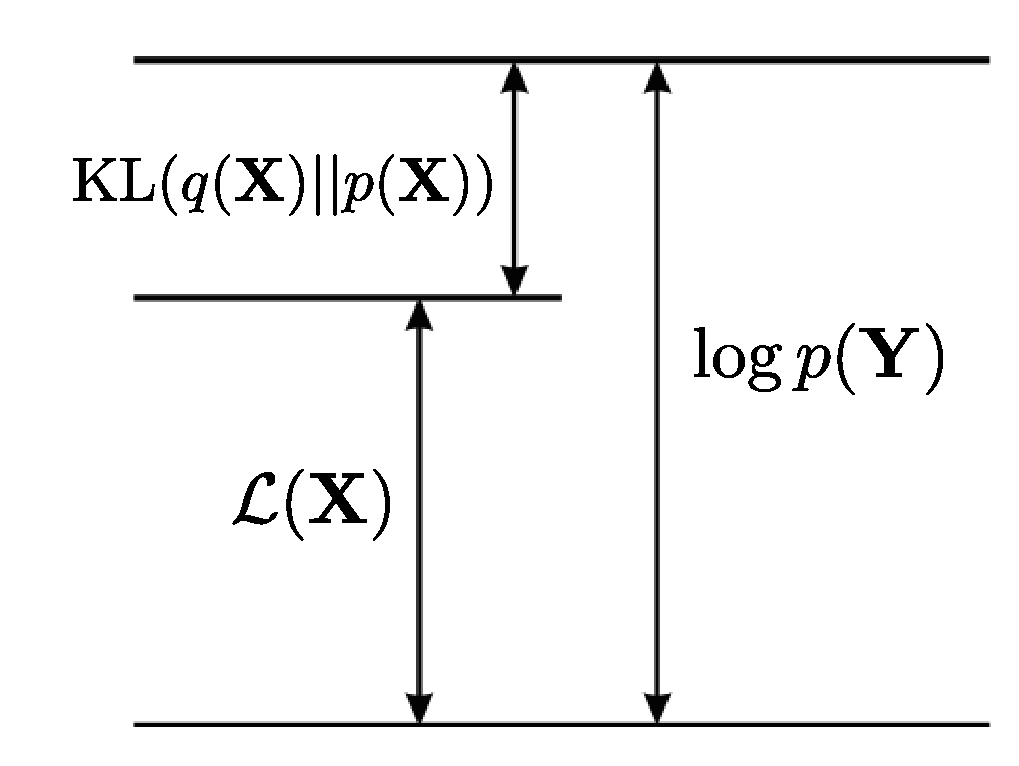
\includegraphics[width=0.35\linewidth]{lower_bound}
	\caption{The quantity $\Lagr(\bfX)$ provides a lower bound on the true log marginal likelihood $\log p(\bfY)$, with the difference being given by the Kullback-Leibler divergence $\KL(q||p)$ between the variational distribution $q(\bfX)$ and the true posterior $p(\bfX|\bfY)$}
	\label{fig:ELBO}
\end{figure}

There are several approaches to define $q(\bfX)$, the two most commonly used are called (unparametric) mean-field and (parametric) fixed-form \cite{Zhang2017,Blei2016}.

\subsubsection{Mean-field variational inference}  \label{section:mean_field}

The most common type of variational Bayes, known as the mean-field approach, assumes that the variational distribution factorises over M disjoint groups of unobserved variables\cite{Saul1996}:
\begin{equation} \label{eq:mean_field}
	q(\bfX) = \prod_{i=1}^{M} q(\bfx_i)
\end{equation}
where typically all unobserved variables are assumed to be independent. Importantly, notice that no parametric assumptions were placed regarding the nature of $q(\bfx_i)$.

Evidently, in sufficiently complex models where the unobserved variables have dependencies this family of distributions do not contain the true posterior (\Cref{fig:mean_field}). Yet, this is a key assumption to obtain an analytical inference scheme that yields surprisingly accurate results \cite{Blei2006,Faes2011,Braun2007}.

\begin{figure}[H]
	\centering
	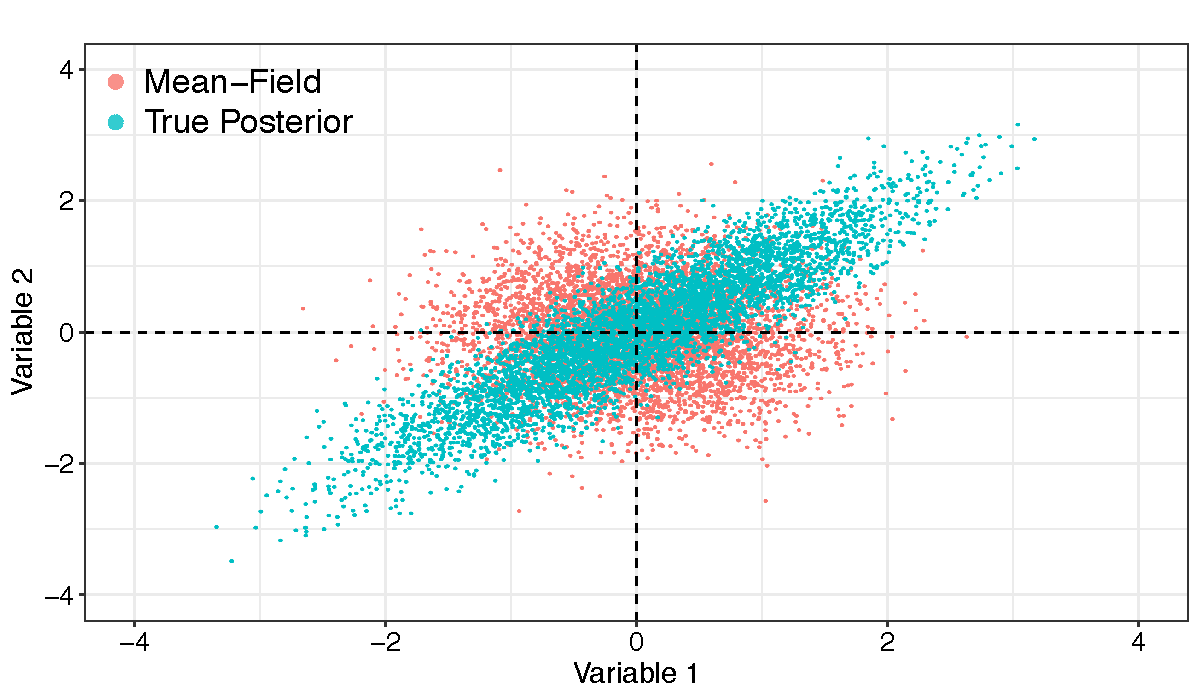
\includegraphics[width=0.7\linewidth]{mean_field}
	\caption{Illustrative example of sampling from a true posterior distribution (blue) versus a fitted mean-field varaitional distribution (red) in a model with two (correlated) unobserved variables. The mean-field approximation wrongly assumes that the unobserved variables are independent.}
	\label{fig:mean_field}
\end{figure}

Using calculus of variations (derivations can be found in \cite{Bishop2006,Murphy}), it follows that the optimal distribution $q(\bfX)$ that maximises the lower bound $\Lagr(\bfX)$ is
\begin{equation} \label{eq:optimal}
	\log \hat{q}_i(\bfx_i) = \E_{-i} [\log p(\bfY,\bfX)] + \mathrm{const}
\end{equation}
where $\E_{-i}$ denotes an expectation with respect to the $q$ distributions over all variables $\bfx_j$ except for $\bfx_i$.\\
The additive constant is set by normalising the distribution $\hat{q}_i(\bfz_i)$:
\[
	\hat{q}(\bfx_i) = \frac{\exp(\E_{-i}[\log p(\bfY,\bfX)])}{\int \exp(\E_{-i}[\log p(\bfY,\bfX)]) d\bfX}
\]
While the form of $\hat{q}(\bfx_i)$ is not restricted to a specific parametric form, it can be shown that when using conjugate priors, the distributions $\hat{q}_i(\bfx_i)$ have the same functional form as the priors $\hat{p}(\bfx_i)$. 
%An example is shown in Appendix X, but a detailed mathematical treatment with derivations of multiple examples can be found in \cite{Bishop2006,Murphy,Zhao2009}.


\subsubsection{Fixed-form variational inference}  \label{section:fixed_form}

An alternative and straightforward choice is to directly define a parametric form for the distribution $q(\bfX)$ with some parameters $\bTheta$. Once the choice of $q(\bfX)$ is made, the parameters $\bTheta$ are optimised to minimise $\KL(q(\bfX)||p(\bfX|\bfY))$ (the variational problem):
\begin{align}
	\hat{\bTheta} &= \argmin_{\bTheta} \KL(q(\bfX)||p(\bfX|\bfY)) \\
	&= \E[\log(q(\bfX)) - \log(p(\bfX,\bfY))]
\end{align}
Numerically optimising this function requires the evaluation of expectations with respect to $q(\bfX)$. In closed form, this is only feasable for a limited group of variational distributions. Alternatively, one can attempt Monte Carlo approximations, but in practice this turns to be slow and leads to high-variance estimates \cite{Braun2007,Ranganath2014,Braun2007}.

Typically, one would choose this distribution to factorise over parameters and to be of the same (exponential) family as the prior $p(\bfX)$. In such case there is a closed form coordinate-ascent scheme available, and it turns out that the fixed-form formulation is equivalent to the (non-parametric) mean-field derivation when using conjugate priors.\\
Unfortunately, for generic models with arbitrary families of distributions, no closed-form variational distributions exist \cite{Zhang2017,Blei2016}. 

However, while the parametric assumption certainly limits the flexibility of variational distributions, the advantage of this formulation is that it opens the possibility to use fast gradient-based methods for the inference procedure \cite{Hoffman2012,Ranganath2014}.

%\paragraph{Black box variational inference}

\subsection{Expectation Propagation}  \label{section:expectation_propagation}

Expectation Propagation (EP) is another deterministic strategy with a similar philosophy as the Variational approach. It is also based on minimising the KL divergence between a variational distribution $q(\bfX)$ and the true posterior $p(\bfX|\bfY)$, but while variational inference minimises $KL(p||q)$, EP maximises the reverse KL-divergence $KL(q||p)$.

Interestingly, this simple difference leads to an inference scheme with stringkly different properties. This can be understood by inspecting the differences between the two KL divergence formulas:

Variational inference:
\begin{equation} \label{eq:kl_vb}
	\KL(q(\bfX)||p(\bfX|\bfY)) = - \int q(\bfX) \log \frac{p(\bfX|\bfY)}{q(\bfX)}
\end{equation}
Expectation propagation:
\begin{equation} \label{eq:kl_ep}
	\KL(p(\bfX|\bfY)||q(\bfX)) = - \int p(\bfX|\bfY) \log \frac{q(\bfX)}{p(\bfX|\bfY)}
\end{equation}
In regions of $\bfX$ where the true posterior density $p(\bfX|\bfY)$ is small, setting a large density for $q(\bfX)$ has a much stronger penalisation in \Cref{eq:kl_ep} than in \Cref{eq:kl_vb}, because of the true posterior density being on the denominator. Hence, EP tends to avoid areas where the density $p(\bfX|\bfY)$ is very low, even if it does not correspond to areas of very high-density in $p(\bfX|\bfY)$. In contrast, in \Cref{eq:kl_vb} there is a strong penalty for having low-density $q(\bfX)$ values.\\
As discussed in \cite{Bishop2006}, the practical consequences of this duality can be observed when the posterior is multi-modal, as in any complex model. In VI, $q(\bfX)$ converges towards areas of high-density in $p(\bfX|\bfY)$, namely local optima. In contrast, EP tends to capture as much non-zero density regions from $p(\bfX|\bfY)$ as possible, thereby averaging across all optima. In the context of doing predictions, the VI solution is much more desirable than the EP solution, as the average of two good parameter values is not necessarily a good value itself.\\
A detailed mathematical treatment of EP, including derivations for specific examples, can be found in \cite{Bishop2006,Murphy,Minka2001}

\begin{figure}[H]
	\centering
	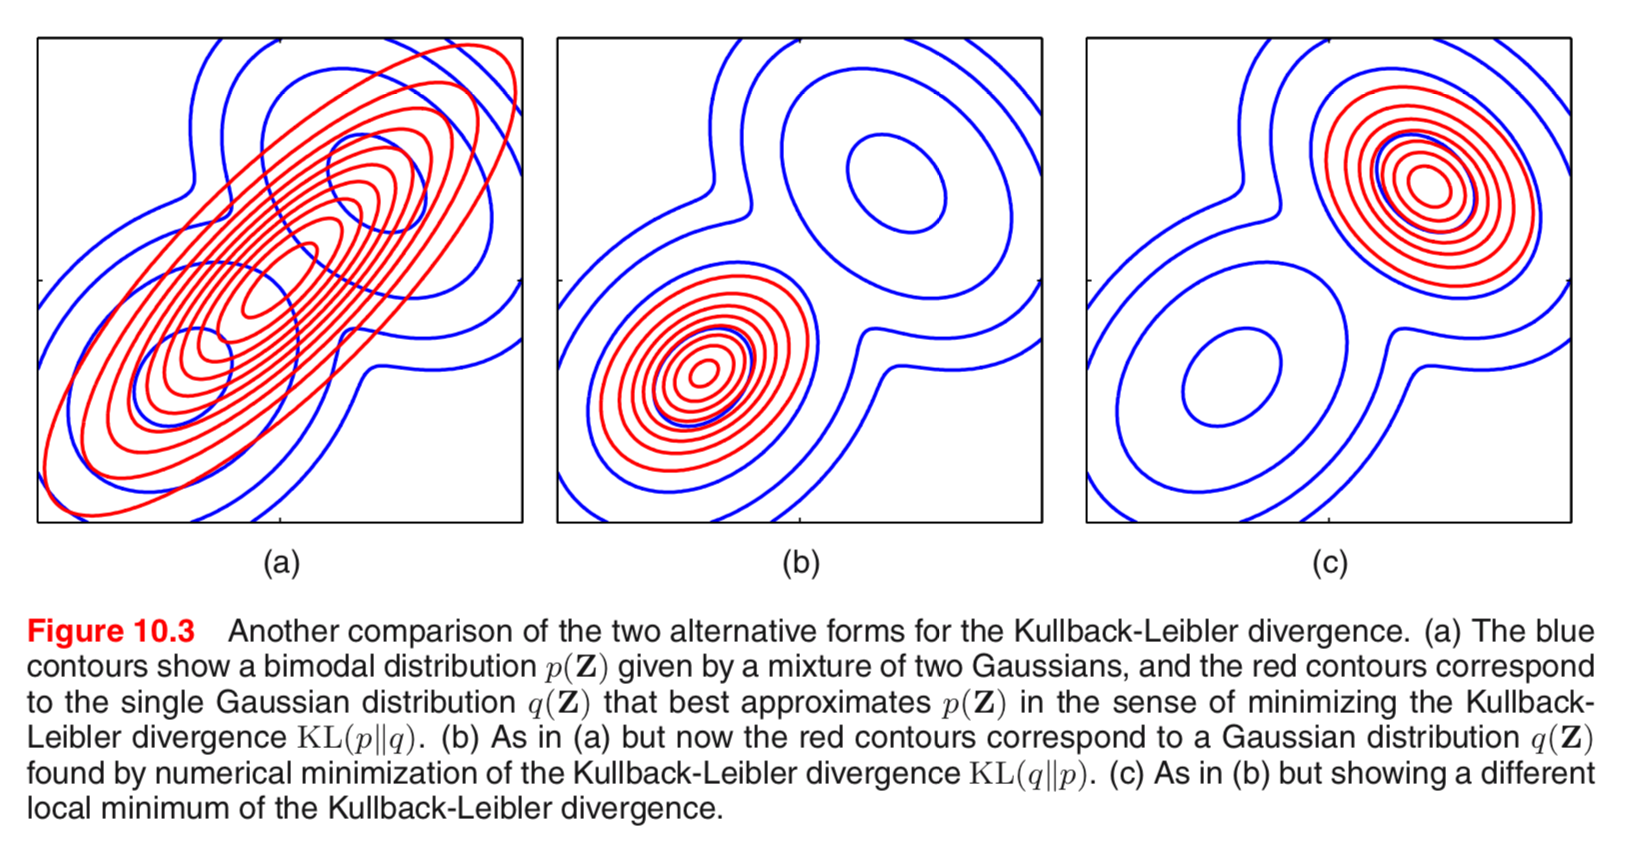
\includegraphics[width=1.0\linewidth]{VB_vs_EP}
	\caption{Illustrative comparison of Variational inference and Expectation Propagation. Shown is the (a) Density and (b) Variance of the true posterior distribution $p(\bfX|\bfY)$ (grey), the variational distribution (orange) and the expectation propagation distribution (green).}
	\label{}
\end{figure}

Following the rationale above, it is easy to predict that variational inference tends to underestimate the variance of the posterior density. Yet, empirical research has shown that this is acceptable, provided that a good model selection is performed \cite{Blei2006}.


\subsubsection{Conclusions}

In this section we have introduced Bayesian modelling and variational inference methods, which will be used later in this chapter.\\
More generally, variational inference is growing in popularity for the analysis of big data sets and it has been applied to a myriad of different problems, including genome-wide association studies \cite{Carbonetto2012}, population genetics, \cite{Raj2014}, network analysis \cite{Sanguinetti2006} and natural language processing \cite{Blei2003}.

Yet, despite its increasing success, there is significant room for improvement. First and foremost, the theoretical guarantees of variational inference are not as developed as in sampling-based MCMC schemes\cite{Blei2016,Zhang2017,Nakajima2007}. As an example, the mean-field setting makes strong independence assumptions about the parameters.  Although it tends to be surprisingly effective, it is not clear in which applications the dependencies between the parameters are important enough that the mean-field approximation could potentially break.\\
More generally, an open research problem is understanding what are the statistical properties of the variational posterior with respect to the exact posterior \cite{Blei2016,Zhang2017}.

As we shall demonstrate later, alternative strategies have been considered to allow some dependencies between the variables, resulting in \textit{structured} mean-field approximations\cite{Hoffman2014,Titsias2011}. However, they often lead to very complex (if not intractable) inference frameworks. 

Finally, another area of extensive research is how to extend the applicability of VI to non-conjugate models. As discussed in \Cref{section:deterministic_bayesian_inference}, the ELBO of non-conjugate models contains intractable integrals, and setting up an inference scheme requires the use of either stochastic Monte Carlo approximations or deterministic approximations that introduce additional lower bounds \cite{Zhang2017,Seeger2012,Khan2017}. In this thesis we follow this rationale to derive an inference framework for a model with non-Gaussian likelihoods.
